\documentclass[11pt,compress,t,notes=noshow, xcolor=table]{beamer}
\documentclass[11pt,compress,t,notes=noshow, xcolor=table]{beamer}
\usepackage[]{graphicx}\usepackage[]{color}
% maxwidth is the original width if it is less than linewidth
% otherwise use linewidth (to make sure the graphics do not exceed the margin)
\makeatletter
\def\maxwidth{ %
  \ifdim\Gin@nat@width>\linewidth
    \linewidth
  \else
    \Gin@nat@width
  \fi
}
\makeatother

\definecolor{fgcolor}{rgb}{0.345, 0.345, 0.345}
\newcommand{\hlnum}[1]{\textcolor[rgb]{0.686,0.059,0.569}{#1}}%
\newcommand{\hlstr}[1]{\textcolor[rgb]{0.192,0.494,0.8}{#1}}%
\newcommand{\hlcom}[1]{\textcolor[rgb]{0.678,0.584,0.686}{\textit{#1}}}%
\newcommand{\hlopt}[1]{\textcolor[rgb]{0,0,0}{#1}}%
\newcommand{\hlstd}[1]{\textcolor[rgb]{0.345,0.345,0.345}{#1}}%
\newcommand{\hlkwa}[1]{\textcolor[rgb]{0.161,0.373,0.58}{\textbf{#1}}}%
\newcommand{\hlkwb}[1]{\textcolor[rgb]{0.69,0.353,0.396}{#1}}%
\newcommand{\hlkwc}[1]{\textcolor[rgb]{0.333,0.667,0.333}{#1}}%
\newcommand{\hlkwd}[1]{\textcolor[rgb]{0.737,0.353,0.396}{\textbf{#1}}}%
\let\hlipl\hlkwb

\usepackage{framed}
\makeatletter
\newenvironment{kframe}{%
 \def\at@end@of@kframe{}%
 \ifinner\ifhmode%
  \def\at@end@of@kframe{\end{minipage}}%
  \begin{minipage}{\columnwidth}%
 \fi\fi%
 \def\FrameCommand##1{\hskip\@totalleftmargin \hskip-\fboxsep
 \colorbox{shadecolor}{##1}\hskip-\fboxsep
     % There is no \\@totalrightmargin, so:
     \hskip-\linewidth \hskip-\@totalleftmargin \hskip\columnwidth}%
 \MakeFramed {\advance\hsize-\width
   \@totalleftmargin\z@ \linewidth\hsize
   \@setminipage}}%
 {\par\unskip\endMakeFramed%
 \at@end@of@kframe}
\makeatother

\definecolor{shadecolor}{rgb}{.97, .97, .97}
\definecolor{messagecolor}{rgb}{0, 0, 0}
\definecolor{warningcolor}{rgb}{1, 0, 1}
\definecolor{errorcolor}{rgb}{1, 0, 0}
\newenvironment{knitrout}{}{} % an empty environment to be redefined in TeX

\usepackage{alltt}
\newcommand{\SweaveOpts}[1]{}  % do not interfere with LaTeX
\newcommand{\SweaveInput}[1]{} % because they are not real TeX commands
\newcommand{\Sexpr}[1]{}       % will only be parsed by R
\newcommand{\xmark}{\ding{55}}%


\usepackage[english]{babel}
\usepackage[utf8]{inputenc}

\usepackage{dsfont}
\usepackage{verbatim}
\usepackage{amsmath}
\usepackage{amsfonts}
\usepackage{amssymb}
\usepackage{bm}
\usepackage{csquotes}
\usepackage{multirow}
\usepackage{longtable}
\usepackage{booktabs}
\usepackage{enumerate}
\usepackage[absolute,overlay]{textpos}
\usepackage{psfrag}
\usepackage{algorithm}
\usepackage{algpseudocode}
\usepackage{eqnarray}
\usepackage{arydshln}
\usepackage{tabularx}
\usepackage{placeins}
\usepackage{tikz}
\usepackage{setspace}
\usepackage{colortbl}
\usepackage{mathtools}
\usepackage{wrapfig}
\usepackage{bm}
\usepackage{amsmath}
\usepackage{pifont}

\usetikzlibrary{shapes,arrows,automata,positioning,calc,chains,trees, shadows}
\tikzset{
  %Define standard arrow tip
  >=stealth',
  %Define style for boxes
  punkt/.style={
    rectangle,
    rounded corners,
    draw=black, very thick,
    text width=6.5em,
    minimum height=2em,
    text centered},
  % Define arrow style
  pil/.style={
    ->,
    thick,
    shorten <=2pt,
    shorten >=2pt,}
}

\usepackage{subfig}

% Defines macros and environments
\usepackage{../../style/lmu-lecture}


\let\code=\texttt
\let\proglang=\textsf

\setkeys{Gin}{width=0.9\textwidth}

\setbeamertemplate{frametitle}{\expandafter\uppercase\expandafter\insertframetitle}

\usepackage{bbm}
% basic latex stuff
\newcommand{\pkg}[1]{{\fontseries{b}\selectfont #1}} %fontstyle for R packages
\newcommand{\lz}{\vspace{0.5cm}} %vertical space
\newcommand{\dlz}{\vspace{1cm}} %double vertical space
\newcommand{\oneliner}[1] % Oneliner for important statements
{\begin{block}{}\begin{center}\begin{Large}#1\end{Large}\end{center}\end{block}}


%new environments
\newenvironment{vbframe}  %frame with breaks and verbatim
{
 \begin{frame}[containsverbatim,allowframebreaks]
}
{
\end{frame}
}

\newenvironment{vframe}  %frame with verbatim without breaks (to avoid numbering one slided frames)
{
 \begin{frame}[containsverbatim]
}
{
\end{frame}
}

\newenvironment{blocki}[1]   % itemize block
{
 \begin{block}{#1}\begin{itemize}
}
{
\end{itemize}\end{block}
}

\newenvironment{fragileframe}[2]{  %fragile frame with framebreaks
\begin{frame}[allowframebreaks, fragile, environment = fragileframe]
\frametitle{#1}
#2}
{\end{frame}}


\newcommand{\myframe}[2]{  %short for frame with framebreaks
\begin{frame}[allowframebreaks]
\frametitle{#1}
#2
\end{frame}}

\newcommand{\remark}[1]{
  \textbf{Remark:} #1
}

\newcommand{\citebutton}[2]{%
\NoCaseChange{\resizebox{!}{9pt}{\protect\beamergotobutton{\href{#2}{#1}}}}%
}



\newenvironment{deleteframe}
{
\begingroup
\usebackgroundtemplate{\includegraphics[width=\paperwidth,height=\paperheight]{../style/color/red.png}}
 \begin{frame}
}
{
\end{frame}
\endgroup
}
\newenvironment{simplifyframe}
{
\begingroup
\usebackgroundtemplate{\includegraphics[width=\paperwidth,height=\paperheight]{../style/color/yellow.png}}
 \begin{frame}
}
{
\end{frame}
\endgroup
}\newenvironment{draftframe}
{
\begingroup
\usebackgroundtemplate{\includegraphics[width=\paperwidth,height=\paperheight]{../style/color/green.jpg}}
 \begin{frame}
}
{
\end{frame}
\endgroup
}
% https://tex.stackexchange.com/a/261480: textcolor that works in mathmode
\makeatletter
\renewcommand*{\@textcolor}[3]{%
  \protect\leavevmode
  \begingroup
    \color#1{#2}#3%
  \endgroup
}
\makeatother





% machine learning
\newcommand{\Xspace}{\mathcal{X}} % X, input space
\newcommand{\Yspace}{\mathcal{Y}} % Y, output space
\newcommand{\nset}{\{1, \ldots, n\}} % set from 1 to n
\newcommand{\pset}{\{1, \ldots, p\}} % set from 1 to p
\newcommand{\gset}{\{1, \ldots, g\}} % set from 1 to g
\newcommand{\Pxy}{\mathbb{P}_{xy}} % P_xy
\newcommand{\Exy}{\mathbb{E}_{xy}} % E_xy: Expectation over random variables xy
\newcommand{\xv}{\mathbf{x}} % vector x (bold)
\newcommand{\xtil}{\tilde{\mathbf{x}}} % vector x-tilde (bold)
\newcommand{\yv}{\mathbf{y}} % vector y (bold)
\newcommand{\xy}{(\xv, y)} % observation (x, y)
\newcommand{\xvec}{\left(x_1, \ldots, x_p\right)^\top} % (x1, ..., xp) 
\newcommand{\Xmat}{\mathbf{X}} % Design matrix
\newcommand{\allDatasets}{\mathds{D}} % The set of all datasets
\newcommand{\allDatasetsn}{\mathds{D}_n}  % The set of all datasets of size n 
\newcommand{\D}{\mathcal{D}} % D, data
\newcommand{\Dn}{\D_n} % D_n, data of size n
\newcommand{\Dtrain}{\mathcal{D}_{\text{train}}} % D_train, training set
\newcommand{\Dtest}{\mathcal{D}_{\text{test}}} % D_test, test set
\newcommand{\xyi}[1][i]{\left(\xv^{(#1)}, y^{(#1)}\right)} % (x^i, y^i), i-th observation
\newcommand{\Dset}{\left( \xyi[1], \ldots, \xyi[n]\right)} % {(x1,y1)), ..., (xn,yn)}, data
\newcommand{\defAllDatasetsn}{(\Xspace \times \Yspace)^n} % Def. of the set of all datasets of size n 
\newcommand{\defAllDatasets}{\bigcup_{n \in \N}(\Xspace \times \Yspace)^n} % Def. of the set of all datasets 
\newcommand{\xdat}{\left\{ \xv^{(1)}, \ldots, \xv^{(n)}\right\}} % {x1, ..., xn}, input data
\newcommand{\yvec}{\left(y^{(1)}, \hdots, y^{(n)}\right)^\top} % (y1, ..., yn), vector of outcomes
\renewcommand{\xi}[1][i]{\xv^{(#1)}} % x^i, i-th observed value of x
\newcommand{\yi}[1][i]{y^{(#1)}} % y^i, i-th observed value of y 
\newcommand{\xivec}{\left(x^{(i)}_1, \ldots, x^{(i)}_p\right)^\top} % (x1^i, ..., xp^i), i-th observation vector
\newcommand{\xj}{\xv_j} % x_j, j-th feature
\newcommand{\xjvec}{\left(x^{(1)}_j, \ldots, x^{(n)}_j\right)^\top} % (x^1_j, ..., x^n_j), j-th feature vector
\newcommand{\phiv}{\mathbf{\phi}} % Basis transformation function phi
\newcommand{\phixi}{\mathbf{\phi}^{(i)}} % Basis transformation of xi: phi^i := phi(xi)

%%%%%% ml - models general
\newcommand{\lamv}{\bm{\lambda}} % lambda vector, hyperconfiguration vector
\newcommand{\Lam}{\bm{\Lambda}}	 % Lambda, space of all hpos
% Inducer / Inducing algorithm
\newcommand{\preimageInducer}{\left(\defAllDatasets\right)\times\Lam} % Set of all datasets times the hyperparameter space
\newcommand{\preimageInducerShort}{\allDatasets\times\Lam} % Set of all datasets times the hyperparameter space
% Inducer / Inducing algorithm
\newcommand{\ind}{\mathcal{I}} % Inducer, inducing algorithm, learning algorithm 

% continuous prediction function f
\newcommand{\ftrue}{f_{\text{true}}}  % True underlying function (if a statistical model is assumed)
\newcommand{\ftruex}{\ftrue(\xv)} % True underlying function (if a statistical model is assumed)
\newcommand{\fx}{f(\xv)} % f(x), continuous prediction function
\newcommand{\fdomains}{f: \Xspace \rightarrow \R^g} % f with domain and co-domain
\newcommand{\Hspace}{\mathcal{H}} % hypothesis space where f is from
\newcommand{\fbayes}{f^{\ast}} % Bayes-optimal model
\newcommand{\fxbayes}{f^{\ast}(\xv)} % Bayes-optimal model
\newcommand{\fkx}[1][k]{f_{#1}(\xv)} % f_j(x), discriminant component function
\newcommand{\fh}{\hat{f}} % f hat, estimated prediction function
\newcommand{\fxh}{\fh(\xv)} % fhat(x)
\newcommand{\fxt}{f(\xv ~|~ \thetab)} % f(x | theta)
\newcommand{\fxi}{f\left(\xv^{(i)}\right)} % f(x^(i))
\newcommand{\fxih}{\hat{f}\left(\xv^{(i)}\right)} % f(x^(i))
\newcommand{\fxit}{f\left(\xv^{(i)} ~|~ \thetab\right)} % f(x^(i) | theta)
\newcommand{\fhD}{\fh_{\D}} % fhat_D, estimate of f based on D
\newcommand{\fhDtrain}{\fh_{\Dtrain}} % fhat_Dtrain, estimate of f based on D
\newcommand{\fhDnlam}{\fh_{\Dn, \lamv}} %model learned on Dn with hp lambda
\newcommand{\fhDlam}{\fh_{\D, \lamv}} %model learned on D with hp lambda
\newcommand{\fhDnlams}{\fh_{\Dn, \lamv^\ast}} %model learned on Dn with optimal hp lambda 
\newcommand{\fhDlams}{\fh_{\D, \lamv^\ast}} %model learned on D with optimal hp lambda 

% discrete prediction function h
\newcommand{\hx}{h(\xv)} % h(x), discrete prediction function
\newcommand{\hh}{\hat{h}} % h hat
\newcommand{\hxh}{\hat{h}(\xv)} % hhat(x)
\newcommand{\hxt}{h(\xv | \thetab)} % h(x | theta)
\newcommand{\hxi}{h\left(\xi\right)} % h(x^(i))
\newcommand{\hxit}{h\left(\xi ~|~ \thetab\right)} % h(x^(i) | theta)
\newcommand{\hbayes}{h^{\ast}} % Bayes-optimal classification model
\newcommand{\hxbayes}{h^{\ast}(\xv)} % Bayes-optimal classification model

% yhat
\newcommand{\yh}{\hat{y}} % yhat for prediction of target
\newcommand{\yih}{\hat{y}^{(i)}} % yhat^(i) for prediction of ith targiet
\newcommand{\resi}{\yi- \yih}

% theta
\newcommand{\thetah}{\hat{\theta}} % theta hat
\newcommand{\thetab}{\bm{\theta}} % theta vector
\newcommand{\thetabh}{\bm{\hat\theta}} % theta vector hat
\newcommand{\thetat}[1][t]{\thetab^{[#1]}} % theta^[t] in optimization
\newcommand{\thetatn}[1][t]{\thetab^{[#1 +1]}} % theta^[t+1] in optimization
\newcommand{\thetahDnlam}{\thetabh_{\Dn, \lamv}} %theta learned on Dn with hp lambda
\newcommand{\thetahDlam}{\thetabh_{\D, \lamv}} %theta learned on D with hp lambda
\newcommand{\mint}{\min_{\thetab \in \Theta}} % min problem theta
\newcommand{\argmint}{\argmin_{\thetab \in \Theta}} % argmin theta

% densities + probabilities
% pdf of x 
\newcommand{\pdf}{p} % p
\newcommand{\pdfx}{p(\xv)} % p(x)
\newcommand{\pixt}{\pi(\xv~|~ \thetab)} % pi(x|theta), pdf of x given theta
\newcommand{\pixit}{\pi\left(\xi ~|~ \thetab\right)} % pi(x^i|theta), pdf of x given theta
\newcommand{\pixii}{\pi\left(\xi\right)} % pi(x^i), pdf of i-th x 

% pdf of (x, y)
\newcommand{\pdfxy}{p(\xv,y)} % p(x, y)
\newcommand{\pdfxyt}{p(\xv, y ~|~ \thetab)} % p(x, y | theta)
\newcommand{\pdfxyit}{p\left(\xi, \yi ~|~ \thetab\right)} % p(x^(i), y^(i) | theta)

% pdf of x given y
\newcommand{\pdfxyk}[1][k]{p(\xv | y= #1)} % p(x | y = k)
\newcommand{\lpdfxyk}[1][k]{\log p(\xv | y= #1)} % log p(x | y = k)
\newcommand{\pdfxiyk}[1][k]{p\left(\xi | y= #1 \right)} % p(x^i | y = k)

% prior probabilities
\newcommand{\pik}[1][k]{\pi_{#1}} % pi_k, prior
\newcommand{\lpik}[1][k]{\log \pi_{#1}} % log pi_k, log of the prior
\newcommand{\pit}{\pi(\thetab)} % Prior probability of parameter theta

% posterior probabilities
\newcommand{\post}{\P(y = 1 ~|~ \xv)} % P(y = 1 | x), post. prob for y=1
\newcommand{\postk}[1][k]{\P(y = #1 ~|~ \xv)} % P(y = k | y), post. prob for y=k
\newcommand{\pidomains}{\pi: \Xspace \rightarrow \unitint} % pi with domain and co-domain
\newcommand{\pibayes}{\pi^{\ast}} % Bayes-optimal classification model
\newcommand{\pixbayes}{\pi^{\ast}(\xv)} % Bayes-optimal classification model
\newcommand{\pix}{\pi(\xv)} % pi(x), P(y = 1 | x)
\newcommand{\pikx}[1][k]{\pi_{#1}(\xv)} % pi_k(x), P(y = k | x)
\newcommand{\pikxt}[1][k]{\pi_{#1}(\xv ~|~ \thetab)} % pi_k(x | theta), P(y = k | x, theta)
\newcommand{\pixh}{\hat \pi(\xv)} % pi(x) hat, P(y = 1 | x) hat
\newcommand{\pikxh}[1][k]{\hat \pi_{#1}(\xv)} % pi_k(x) hat, P(y = k | x) hat
\newcommand{\pixih}{\hat \pi(\xi)} % pi(x^(i)) with hat
\newcommand{\pikxih}[1][k]{\hat \pi_{#1}(\xi)} % pi_k(x^(i)) with hat
\newcommand{\pdfygxt}{p(y ~|~\xv, \thetab)} % p(y | x, theta)
\newcommand{\pdfyigxit}{p\left(\yi ~|~\xi, \thetab\right)} % p(y^i |x^i, theta)
\newcommand{\lpdfygxt}{\log \pdfygxt } % log p(y | x, theta)
\newcommand{\lpdfyigxit}{\log \pdfyigxit} % log p(y^i |x^i, theta)

% probababilistic
\newcommand{\bayesrulek}[1][k]{\frac{\P(\xv | y= #1) \P(y= #1)}{\P(\xv)}} % Bayes rule
\newcommand{\muk}{\bm{\mu_k}} % mean vector of class-k Gaussian (discr analysis) 

% residual and margin
\newcommand{\eps}{\epsilon} % residual, stochastic
\newcommand{\epsi}{\epsilon^{(i)}} % epsilon^i, residual, stochastic
\newcommand{\epsh}{\hat{\epsilon}} % residual, estimated
\newcommand{\yf}{y \fx} % y f(x), margin
\newcommand{\yfi}{\yi \fxi} % y^i f(x^i), margin
\newcommand{\Sigmah}{\hat \Sigma} % estimated covariance matrix
\newcommand{\Sigmahj}{\hat \Sigma_j} % estimated covariance matrix for the j-th class

% ml - loss, risk, likelihood
\newcommand{\Lyf}{L\left(y, f\right)} % L(y, f), loss function
\newcommand{\Lxy}{L\left(y, \fx\right)} % L(y, f(x)), loss function
\newcommand{\Lxyi}{L\left(\yi, \fxi\right)} % loss of observation
\newcommand{\Lxyt}{L\left(y, \fxt\right)} % loss with f parameterized
\newcommand{\Lxyit}{L\left(\yi, \fxit\right)} % loss of observation with f parameterized
\newcommand{\Lxym}{L\left(\yi, f\left(\bm{\tilde{x}}^{(i)} ~|~ \thetab\right)\right)} % loss of observation with f parameterized
\newcommand{\Lpixy}{L\left(y, \pix\right)} % loss in classification
\newcommand{\Lpixyi}{L\left(\yi, \pixii\right)} % loss of observation in classification
\newcommand{\Lpixyt}{L\left(y, \pixt\right)} % loss with pi parameterized
\newcommand{\Lpixyit}{L\left(\yi, \pixit\right)} % loss of observation with pi parameterized
\newcommand{\Lhxy}{L\left(y, \hx\right)} % L(y, h(x)), loss function on discrete classes
\newcommand{\Lr}{L\left(r\right)} % L(r), loss defined on residual (reg) / margin (classif)
\newcommand{\lone}{|y - \fx|} % L1 loss
\newcommand{\ltwo}{\left(y - \fx\right)^2} % L2 loss
\newcommand{\lbernoullimp}{\ln(1 + \exp(-y \cdot \fx))} % Bernoulli loss for -1, +1 encoding
\newcommand{\lbernoullizo}{- y \cdot \fx + \log(1 + \exp(\fx))} % Bernoulli loss for 0, 1 encoding
\newcommand{\lcrossent}{- y \log \left(\pix\right) - (1 - y) \log \left(1 - \pix\right)} % cross-entropy loss
\newcommand{\lbrier}{\left(\pix - y \right)^2} % Brier score
\newcommand{\risk}{\mathcal{R}} % R, risk
\newcommand{\riskbayes}{\mathcal{R}^\ast}
\newcommand{\riskf}{\risk(f)} % R(f), risk
\newcommand{\riskdef}{\E_{y|\xv}\left(\Lxy \right)} % risk def (expected loss)
\newcommand{\riskt}{\mathcal{R}(\thetab)} % R(theta), risk
\newcommand{\riske}{\mathcal{R}_{\text{emp}}} % R_emp, empirical risk w/o factor 1 / n
\newcommand{\riskeb}{\bar{\mathcal{R}}_{\text{emp}}} % R_emp, empirical risk w/ factor 1 / n
\newcommand{\riskef}{\riske(f)} % R_emp(f)
\newcommand{\risket}{\mathcal{R}_{\text{emp}}(\thetab)} % R_emp(theta)
\newcommand{\riskr}{\mathcal{R}_{\text{reg}}} % R_reg, regularized risk
\newcommand{\riskrt}{\mathcal{R}_{\text{reg}}(\thetab)} % R_reg(theta)
\newcommand{\riskrf}{\riskr(f)} % R_reg(f)
\newcommand{\riskrth}{\hat{\mathcal{R}}_{\text{reg}}(\thetab)} % hat R_reg(theta)
\newcommand{\risketh}{\hat{\mathcal{R}}_{\text{emp}}(\thetab)} % hat R_emp(theta)
\newcommand{\LL}{\mathcal{L}} % L, likelihood
\newcommand{\LLt}{\mathcal{L}(\thetab)} % L(theta), likelihood
\newcommand{\LLtx}{\mathcal{L}(\thetab | \xv)} % L(theta|x), likelihood
\newcommand{\logl}{\ell} % l, log-likelihood
\newcommand{\loglt}{\logl(\thetab)} % l(theta), log-likelihood
\newcommand{\logltx}{\logl(\thetab | \xv)} % l(theta|x), log-likelihood
\newcommand{\errtrain}{\text{err}_{\text{train}}} % training error
\newcommand{\errtest}{\text{err}_{\text{test}}} % test error
\newcommand{\errexp}{\overline{\text{err}_{\text{test}}}} % avg training error

% lm
\newcommand{\thx}{\thetab^\top \xv} % linear model
\newcommand{\olsest}{(\Xmat^\top \Xmat)^{-1} \Xmat^\top \yv} % OLS estimator in LM 



%\newcommand{\titlefigure}{} MISSING
%\newcommand{\learninggoals}{
%  \item \textcolor{blue}{XXXXXXXXXXXXXXXX}
%  \item \textcolor{blue}{XXXXXXXXXXXXXXXX}
%}

\title{Introduction to Machine Learning}
% \author{Bernd Bischl, Christoph Molnar, Daniel Schalk, Fabian Scheipl}
\institute{\href{https://compstat-lmu.github.io/lecture_i2ml/}{compstat-lmu.github.io/lecture\_i2ml}}
\date{}

\setbeamertemplate{frametitle}{\expandafter\uppercase\expandafter\insertframetitle}



\begin{document}


\lecturechapter{The Two Cultures of Statistical Modeling}
\lecture{Introduction to Machine Learning}

  
% \begin{vbframe}{Modeling: two cultures}
% \begin{center}
% <<fig.height=3, fig.width=12>>=
% grid.newpage()
% pushViewport(viewport(x = 0.1, y = 0.5, width = 0.14, height = 0.56, angle = 45))
% grid.rect(gp = gpar(lwd = 4))
% grid.text("x", rot = -45, gp = gpar(fontsize = 24, fontface = "bold"))
% popViewport()
% pushViewport(viewport(x = 0.5, y = 0.5, width = 0.4, height = 0.8, angle = 0))
% grid.rect(gp = gpar(lwd = 4))
% grid.text("System", gp = gpar(fontsize = 24, fontface = "bold"))
% popViewport()
% pushViewport(viewport(x = 0.9, y = 0.5, width = 0.14, height = 0.56, angle = 45))
% grid.rect(gp = gpar(lwd = 4))
% grid.text("y", rot = -45, gp = gpar(fontsize = 24, fontface = "bold"))
% popViewport()
% grid.lines(c(0.1 + sqrt(2*0.07^2), 0.3), rep(0.5, 2), arrow = arrow(length = unit(0.2, "inch"), type = "closed"),
%            gp = gpar(lwd = 4))
% grid.lines(c(0.7, 0.9 - sqrt(2*0.07^2)), rep(0.5, 2), arrow = arrow(length = unit(0.2, "inch"), type = "closed"),
%            gp = gpar(lwd = 4))
% @
% \end{center}
% System: nature, organism, chemical reaction, technical process, human behavior, \ldots
% \end{vbframe}
%
% \begin{vbframe}{two cultures: classical statistics}
% We assume that one can sufficiently describe the unknown system by the stochastic model
% $$y = f(x, \theta) + \epsilon$$
% and a \emph{parametric} function class for $f()$ is given. \\
% \lz
% \emph{Under the assumption} that the model is correct, now the usual operation of statistical inference can be built up:
% \begin{itemize}
%  \item Hypothesis tests, variance analysis, model comparison
%  \item Confidence intervals for parameters and predictions
% \end{itemize}
%
% \newpage
% Many articles in JASA, the Annals of Statistics etc. start with
% \enquote{Assume that the data are generated by the following model \ldots}.
%
% \begin{itemize}
% \item \textbf{Advantages:}
%   \begin{itemize}
%   \item Parameter can be interpreted if the model is easy enough
%   \item Good theory for model diagnostics
%   \end{itemize}
%  \item \textbf{Disadvantages (Breiman 2001):}
%    \begin{itemize}
%   \item \enquote{irrelevant theory}
%   \item \enquote{questionable scientific conclusions}
%   \end{itemize}
% \end{itemize}
% \end{vbframe}
%
% \begin{vbframe}{Two cultures: machine learning}
% \begin{center}
% <<fig.height=6, fig.width=12>>=
% grid.newpage()
% pushViewport(viewport(x = 0.1, y = 0.75, width = 0.14, height = 0.28, angle = 45))
% grid.rect(gp = gpar(lwd = 4))
% grid.text("x", rot = -45, gp = gpar(fontsize = 24, fontface = "bold"))
% popViewport()
% pushViewport(viewport(x = 0.5, y = 0.75, width = 0.4, height = 0.4, angle = 0))
% grid.rect(gp = gpar(lwd = 4))
% grid.text("System", gp = gpar(fontsize = 24, fontface = "bold"))
% popViewport()
% pushViewport(viewport(x = 0.9, y = 0.75, width = 0.14, height = 0.28, angle = 45))
% grid.rect(gp = gpar(lwd = 4))
% grid.text("y", rot = -45, gp = gpar(fontsize = 24, fontface = "bold"))
% popViewport()
% grid.lines(c(0.1 + sqrt(2*0.07^2), 0.3), rep(0.75, 2), arrow = arrow(length = unit(0.2, "inch"), type = "closed"),
%            gp = gpar(lwd = 4))
% grid.lines(c(0.7, 0.9 - sqrt(2*0.07^2)), rep(0.75, 2), arrow = arrow(length = unit(0.2, "inch"), type = "closed"),
%            gp = gpar(lwd = 4))
% grid.roundrect(0.5, 0.2, 0.7, 0.3, name = "rr", gp = gpar(lwd = 4))
% grid.text("Approximation by\nneuronal network, tree, ...", y = 0.2,
%           gp = gpar(fontsize = 24, fontface = "bold"))
% grid.curve(0.1, 0.55, 0.15, 0.2,
%    arrow = arrow(length = unit(0.2, "inch"), type = "closed"),
%    gp = gpar(lwd = 4))
% grid.curve(0.85, 0.2, 0.9, 0.55,
%    arrow = arrow(length = unit(0.2, "inch"), type = "closed"),
%    gp = gpar(lwd = 4))
% @
% \end{center}
% The system is considered as unknown, explicit modelling is not even tried.
% Essential measure of goodness is the prediction quality.
%
% \framebreak
%
% Use of methods which are able to model many systems (universal approximations), development of methods by examples of nature, intuitive behavioral or because of computational attractivity.
% \vspace{0.25cm}
% \begin{itemize}
%  \item \textbf{Advantages:}
%    \begin{itemize}
%    \item Many more model classes are available, much quicker development and implementation of new ideas.
%    \item For predictions, knowledge about the distribution of the parameters,
%    diligent task, knowledge about the error distribution is sufficient.
%    \end{itemize}
%  \item \textbf{Disadvantages:}
%    \begin{itemize}
%    \item Models are mostly hard to interpret (\enquote{black box})
%    \end{itemize}
% \end{itemize}
% \vspace{0.25cm}
% Many models which originally come from machine learning are also statistical mainstream nowadays (and have in parts been considerably improved).


\begin{vbframe}{Modeling: two cultures}
\textbf{Statistics, the Data Modeling Culture}
\begin{center}
\vspace{1cm}
  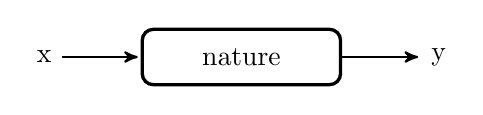
\begin{tikzpicture}[->,>=stealth',shorten >=1pt,auto,node distance=1cm,
      thick,main node/.style={circle,fill=blue!20,draw,font=\sffamily\Large\bfseries}]
    \node[punkt] (nature) {nature};
    \node[left=of nature] (x) {x};
    \node[right=of nature] (y) {y};
    \path[every node/.style={font=\sffamily\small}]
    (nature) edge node {} (y)
    (x) edge node  {} (nature)
    ;
  \end{tikzpicture} \\
\vspace{1cm}
\begin{itemize}
  \item In a strongly simplified world an arbitrary outcome $y$ is produced by \enquote{nature} from the features given in $x$
  \item The knowledge about nature's true mechanisms ranges from entirely unknown (or stochastic) to established (scientific), possibly deterministic explanations
  %\item Example: Outcome $y$ is the rent for apartments and covariates $x$ are size, number of bathrooms and location
\end{itemize}
\end{center}

\framebreak

\begin{itemize}
  \item Focus on the modeling of data, which can be reduced to two targets:
  \begin{enumerate}
    \item Learn a model to predict the outcome for new covariates
    \item Get a better understanding about the relationship between covariates and outcome
  \end{enumerate}
\end{itemize}
\begin{center}
    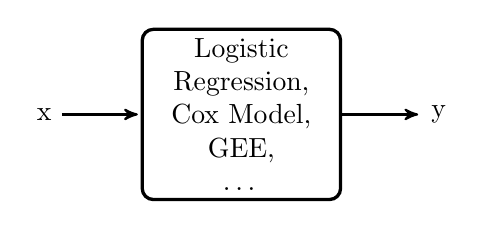
\begin{tikzpicture}[->,>=stealth',shorten >=1pt,auto,node distance=1cm,
        thick,main node/.style={circle,fill=blue!20,draw,font=\sffamily\Large\bfseries}]
      \node[punkt] (natur) {Logistic Regression, \\Cox Model, \\GEE, \\ \ldots};
      \node[left=of natur] (x) {x};
      \node[right=of natur] (y) {y};
      \path[every node/.style={font=\sffamily\small}]
      (natur) edge node {} (y)
      (x) edge node  {} (natur)
      ;
    \end{tikzpicture}
  \end{center}
\begin{itemize}
  \item Find a stochastic model of the data-generating process:
  $$y = f(x, \text{parameters}, \text{random error})$$
\end{itemize}

\framebreak

In this \enquote{data modeling culture}, a stochastic model for the data- generating process is assumed
\begin{blocki}{Typical assumptions and restrictions}
  \item Specific stochastic model that generated the data
  \item Distribution of residuals
  \item Linearity, additivity (e.g. linear predictor)
  \item Manual specification of interactions
\end{blocki}

\framebreak

\textbf{Machine Learning, the Algorithmic Modeling Culture}
\lz
  \begin{center}
    \begin{tikzpicture}[->,>=stealth',shorten >=1pt,auto,node distance=1cm,
        thick,main node/.style={circle,fill=blue!20,draw,font=\sffamily\Large\bfseries}]
      \node[punkt] (natur) {unknown};
      \node[left=of natur] (x) {x};
      \node[right=of natur] (y) {y};
      \node[below=of natur, label=below:algorithm] (algo) {\includegraphics[width = 3cm]{figure_man/machine.png}};
      \path[every node/.style={font=\sffamily\small}]
      (natur) edge node {} (y)
      (x) edge node  {} (natur)
      (x) edge[<->, bend right=30] node {} (algo)
      (y) edge[<->, bend left=30] node {} (algo)
      ;
    \end{tikzpicture}
  \end{center}
\lz
Find a function $\fx$ that minimizes the loss: $\Lxy$

\framebreak

\begin{itemize}
  \item In the \enquote{algorithmic modeling culture}, the true mechanism is treated as unknown
  \item The goal is not finding the true data-generating process but developing an algorithm that imitates/predicts (specific aspects of) a data-generating process as closely as possible
  \item Modeling is reduced to a mere problem of function optimization: Given the covariates $x$, outcome $y$ and a loss function, find a function $\fx$ which minimizes the loss for the prediction of the outcome
\end{itemize}
\begin{blocki}{Algorithm in Machine Learning}
  \item Boosting
  \item Support Vector Machines
  \item Artificial neural networks
  \item Random Forests
  \item Hidden Markov
  \item Bayes-Nets
  \item \ldots
\end{blocki}

\end{vbframe}

\begin{vbframe}{Prediction vs. Interpretation}
\vspace{1.5cm}
\begin{center}
  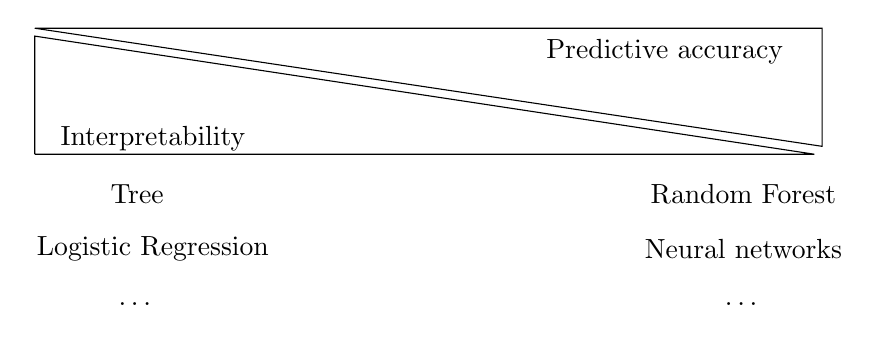
\begin{tikzpicture}
    \draw (0,0) -- (0,1.5) -- (9.9,0) -- (0,0);
    \draw  (0, 1.6) -- (10,1.6) -- (10, 0.1) -- (0, 1.6);
    \node at (1.5, 0.2) {Interpretability};
    \node at (8, 1.3) {Predictive accuracy};
    \node at (1.3, -0.5) {Tree};
    \node at (9, -0.5) {Random Forest};
    \node at (1.5, -1.2) {Logistic Regression};
    \node at (9, -1.2) {Neural networks};
    \node at (1.3, -1.9) {\ldots};
    \node at (9, -1.9) {\ldots};
  \end{tikzpicture}
\end{center}

\framebreak

\begin{itemize}
  \item There is a trade-off between interpretability and predictive accuracy: models that yield accurate predictions are often complex and models that are easy to interpret are often bad predictors
  \lz
  \item Example logistic regression and $k$ Nearest Neighbors: in LR, we can inspect each coefficient and understand how changes in a single feature affect the class probabilities. kNN offers no such interpretability, but if the class boundaries are very nonlinear, it will have much better predictive accuracy.
\end{itemize}

\end{vbframe}

\begin{frame}{Dimensionality of the data}
\begin{blocki}{}
  \item The higher the dimensionality of the data (\# covariates) the more difficult is the separation of signal and noise
  \item Common practice in data modeling: variable selection (by expert selection or data driven) and reduction of dimensionality (e.g. PCA)
  \item Common practice in algorithmic modeling: Engineering of new features (covariates) to increase predictive accuracy; algorithms robust for many covariates
\end{blocki}

\end{frame}

\begin{vbframe}{Modeling: Two Cultures}

\begin{blocki}{Problems and Blindspots of Data Modeling Culture:}
  \item Conclusions about assumed model are interpreted as being about nature (reification).
  \item Model assumptions often violated.
  \item Often improper model evaluation presuming model validity\\
  $\Rightarrow$ can lead to irrelevant theory and questionable statistical conclusions
  \item Data models fail in areas like image and speech recognition
\end{blocki}

\framebreak

\begin{blocki}{Problems and Blindspots of Algorithmic Modeling Culture:}
  \item Uncertainty quantification often difficult / impossible, almost always an afterthought.
  \item Models are often uninterpretable \enquote{black boxes}: \\
  $\Rightarrow$ Can you trust something you don't understand?
  \item Often ignores suitable sampling plans or issues with data provenance that can jeopardize generalizability
\end{blocki}

% \framebreak
%
% \begin{blocki}{Goodness of model}
%   \item Data modeling culture: Evaluation of goodness of fit often based on model assumptions (e.g. Likelihood) and calculated on training data
%   \item Algorithmic modeling culture: Evaluation of predictive accuracy with an extra test set or cross validation (more later)
% \end{blocki}
%
% How good is a statistical model if the predictive accuracy is weak?\\
% Are interpretations of parameters and p-values legitimate?


\framebreak
Different terminology for machine learning and statistics:

\begin{small}
  \begin{table}
    \begin{tabular}{lr}
      \hline
      Machine Learning & Statistics \\
      \hline
      Feature, Attribute & Covariate \\
      Label & Response \\
      Example, Instance & Observation \\[.3em]

      Weight & Parameter, Coefficient \\
      Bias term & Intercept \\[.3em]

      Minimizing loss & Maximizing likelihood / Estimating posterior \\
      Learning & Fitting, Estimation \\
      Hypothesis & (Fitted) Model \\
      Learner & Model (Class) \\[.3em]

      Supervised Learning & Regression / Classification \\
      Unsupervised Learning & Density estimation / Clustering\\
      Data Mining (good) & Data Mining (bad)\\
    \end{tabular}
  \end{table}
  \end{small}
  {\scriptsize{see also: \url{https://ubc-mds.github.io/resources_pages/terminology}}}

\framebreak

\lz
\structure{Summary}\\

Data modeling culture: \enquote{The model is true.}\\

\emph{Tries to estimate stochastic properties of the true data-generating process and focuses on parameters and their uncertainty.}\\
\vspace{1cm}

Algorithmic modeling culture: \enquote{The model is useful.}\\

\emph{Tries to minimize some measure of divergence between observations from the data-generating process and a function that imitates its behavior and focuses on predictive accuracy.}\\
\vspace{1cm}

These are broad generalizations, there is much overlap and synergy between the two perspectives.

\framebreak

\structure{Rashomon Effect}\\

\lz

\emph{In practice, many different models often describe a given set of data equally well, which makes it difficult to identify a \enquote{true} data-generating process. \\
\lz\lz

In practice, using different loss functions / evaluation schemes will yield different optimal models, which makes it difficult to identify the \enquote{most useful} model.}

\end{vbframe}

\begin{vbframe}{Parameters, Statistics and Supervised Machine Learning}

\begin{itemize}
\item Supervised ML additionally assumes that $f$ is of a certain \enquote{form}
or comes from a certain \emph{class of functions}.\\
This is necessary to make the problem of automatically finding a \enquote{good} model feasible at all.
\item The specific behavior of a mapping from this class can then be described by \textbf{parameters} which defines its shape.
\item Statistics also studies how to learn such functions (or, rather: their parameters) from example data and how to perform inference on them and interpret the results.
\item For historical reasons, statistics is mostly focused on fairly simple classes of mappings, like (generalized) linear models.
\item Supervised ML also includes more complex kinds of mappings that can often deal with more complicated and high-dimensional inputs.
\end{itemize}
\end{vbframe}

\endlecture
\end{document}
